\documentclass[10pt]{exam}
\usepackage{mathtools}
\usepackage{sansmath}
\usepackage{xfrac}
\usepackage{amssymb}
\usepackage{float}
\usepackage[colorlinks,urlcolor=cyan!60!black]{hyperref}
\usepackage{cleveref}
\usepackage{enumitem}
\usepackage{cancel}
\usepackage{tikz}
\usepackage{algorithm}
\usepackage{algorithmicx}
\usepackage{algpseudocode}
\usepackage{listings}
\usepackage{xcolor}

% Thanks to: https://tex.stackexchange.com/a/75406/69346
\usepackage[outline]{contour}
\usepackage{ulem}
\normalem % use classical emph

\newcommand \myul[4]{%
  \begingroup%
  \renewcommand \ULdepth {#1}%
  \renewcommand \ULthickness {#2}%
  \contourlength{#3}%
  \uline{\phantom{#4}}\llap{\contour{white}{#4}}%
  \endgroup%
}

\newcommand \myulline[4]{%
  \begingroup%
  \renewcommand \ULdepth {#1}%
  \renewcommand \ULthickness {#2}%
  \contourlength{#3}%
  \noindent\rlap{\uline{\hspace{\textwidth}}}\contour{white}{#4}%
  \endgroup%
}

\newcommand\undline[1]{\myul{2pt}{0.5pt}{1pt}{#1}}

%%% A minipage modification that respects parskips
\newlength{\currentparskip}
\newenvironment{minipageparskip}[1]
{\setlength{\currentparskip}{\parskip}% save the value
	\begin{minipage}[b]{#1}% open the minipage
		\setlength{\parskip}{\currentparskip}% restore the value
	}
{\end{minipage}}

%%% Mathematical tools
\DeclarePairedDelimiter{\ceil}{\lceil}{\rceil}
\DeclarePairedDelimiter{\floor}{\lfloor}{\rfloor}

\DeclareMathOperator{\OH}{\mathit{O}}
\DeclareMathOperator{\oh}{\mathit{o}}
\DeclareMathOperator{\OMEGA}{\mathit{\Omega}}
\DeclareMathOperator{\THETA}{\mathit{\Theta}}
\DeclareMathOperator{\SIM}{\mathit{\sim}}

\newcommand{\es}{\varnothing}

%%% Exam layout specifications
\pointname{ pts}
\pointformat{\bfseries (\thepoints)}
\renewcommand\partshook{\setlength\parsep{2ex}}

\pagestyle{headandfoot}
\firstpagefooter{}{Page \thepage\ of \numpages}{}
\runningfooter{}{Page \thepage\ of \numpages}{}

%%% Commands for the answering spaces
\newcommand{\cc}{\fillin[X][0.5cm]}
\newcommand\answerspace{}
\newcommand\drawspace{
	{
	\vspace*{1.6cm}~
	\begin{center}
		\emph{
			You are allowed to draw this by hand.\\
			Make sure that your writing is clear!
		}
	\end{center}~
	\vspace*{1.6cm}
	}
}

\newcommand\answerAA\answerspace
\newcommand\answerAB\answerspace
\newcommand\answerAC\answerspace
\newcommand\answerBA\answerspace
\newcommand\answerBB\answerspace
\newcommand\answerBC\answerspace
% \input{./ans/ans.tex}

\title{
	\vspace*{-2em}
	Cmpe 300: Homework 3 --- 
	Due: December 30th 17:00
}
\author{}
\date{}

%%% Replace these to write your Name and ID into header: vvvvvvvvvvvvvvv
\firstpageheader{Due: Dec 30 17:00}{}{Name and ID: Ibrahim Ozgurcan Oztas, 2016400198}

\begin{document}

\maketitle
\thispagestyle{headandfoot}

\vspace*{-4.5em}
\begin{center}
\fbox{%
\setlength{\fboxsep}{1.9ex}%
\fbox{%
\parbox{0.9\textwidth}{%
	The purpose of this homework is to familiarize you
	with algorithm analysis.
	Solve the following questions
	in \LaTeX{} or using a word processor.
	Submit your solutions \undline{to Moodle as a PDF.}
	\href{https://www.cmpe.boun.edu.tr/~gungort/informationstudents.htm}{Due date is strict.}
	You do not have to print the questions.
	Your answers need not be on separate pages.

	\vspace*{0.7ex}

	\begin{itemize}[noitemsep,nolistsep]
		\item
			This is an individual assignment, so work on your own.
		\item
			Please do not submit just an answer,
			and rather show all your reasoning.
		\item
			For any further questions, contact the assistant
			at \href{mailto:utkan.gezer@boun.edu.tr}{utkan.gezer@boun.edu.tr}.
	\end{itemize}
}}}
\end{center}
\vspace*{2ex}

\begin{questions}
	\question[50]
	Solve the following parts concerning the figure to the right.
	
	\begin{minipageparskip}{0.65\textwidth}
		\vspace{1ex}
		\paragraph{Description of the figure}
		The side length of the square is 1 unit.
		There are 4 quarter-circles at each corner.
		They each have a radius of 1 unit.
		The blue area is the intersection of those
		quarter-circles.
		\vspace{0ex}
	\end{minipageparskip}
	\hfill
	\begin{minipage}[b]{0.25\textwidth}
	\begin{figure}[H]
		\hspace{5ex}
		\begin{tikzpicture}[overlay,scale=2]
			\foreach \x/\a in {0/east,1/west} \foreach \y in {0,1} {
				\node [anchor=\a] at (\x,\y) {$(\x,\y)$};
				\fill (\x,\y) circle (0.04);
			}
			\draw (0,0) rectangle (1,1);
			\clip (0,0) rectangle (1,1);
			\foreach \x in {0,1} \foreach \y in {0,1} \draw (\x,\y) circle (1);
			\foreach \x in {0,1} \foreach \y in {0,1} \clip (\x,\y) circle (1);
			\fill [cyan!90!black] (0,0) rectangle (1,1);
		\end{tikzpicture}
	\end{figure}
	\end{minipage}
	\vspace{3ex}


	\begin{parts}
		\part
		Write a numerical probabilistic algorithm approximating the blue area in the figure.

		\textbf{Hint}\hspace{1ex}
		Write an inequality for the circular areas
		centered at each corner.
		A point satisfying all of those inequalities
		is a point in the blue area, and vice versa.

		\paragraph{Answer\\}
		The function below evaluates whether the point is in the blue area or not, by checking the boundary conditions of four quarter circle.
		\begin{algorithmic}
		\Function{IsIn}{x, y}
		\If{$x^2+y^2 < 1 \wedge (x-1)^2 + y^2 < 1 \wedge x^2 + (y-1)^2 < 1 \wedge (x-1)^2 + (y-1)^2 < 1$} \\
		\hspace{1cm}\Return true
		\Else \\
		\hspace{1cm}\Return false 
		\EndIf
		\EndFunction \\\\
		The function below evaluates the sample to analyze the points that rest in blue area, and returns the percentage of those who rest in blue area.
		\Function{NumericalProb}{$IsIn, x, y, Q$} \\
		\hspace{0.5cm}$success\leftarrow0$ \\
		\hspace{0.5cm}$i\leftarrow0$
		\For{$i$ \textbf{to} Q} \\
		\hspace{1cm} $call Random(\{0, ..., 1\}, x)$ \\
		\hspace{1cm} $call Random(\{0, ..., 1\}, y)$
		\hspace{1cm} \If{$IsIn(x, y)$} \\
		\hspace{1.5cm} $success \leftarrow success + 1$
		\EndIf
		\EndFor \\
		\Return $success * 100$ / $Q$ 
		\EndFunction
		\end{algorithmic}
		\vfill
		
		\newpage
		\part
		Generate 10 random points within the square ($x, y$ pairs between 0 and 1)
		using your favorite programming language or the
		\href{https://www.random.org/decimal-fractions/}{Random Decimal Fraction Generator of
		Random.org}.
		
		\paragraph{Answer\\}
		$Point1=(0.530324, 0.131470)$ \hspace{0.1cm} $Point2=(0.427873, 0.840549)$ \hspace{0.1cm} $Point3=(0.911731, 0.560807)$ \\
		$Point4=(0.993659, 0.225091)$ \hspace{0.1cm}
		$Point5=(0.164563, 0.522170)$ \hspace{0.1cm} $Point6=(0.807351, 0.124272)$ \\ 
		$Point7=(0.637379, 0.421693)$ \hspace{0.1cm} $Point8=(0.343053, 0.717368)$ \hspace{0.1cm}
		$Point9=(0.929043, 0.377408)$ \\ 
		$Point10=(0.539279, 0.457904)$ \hspace{0.1cm} $Point11=(0.799350, 0.391014)$ \hspace{0.1cm} $Point12=(0.029634, 0.570495)$ \\
		$Point13=(0.535416, 0.203938)$ \hspace{0.1cm} $Point14=(0.570168, 0.518679)$ \hspace{0.1cm} $Point15=(0.493724, 0.511799)$ \\ 
		$Point16=(0.025889, 0.024048)$ \hspace{0.1cm}
		$Point17=(0.643269, 0.453762)$ \hspace{0.1cm} $Point18=(0.864597, 0.555001)$ \\ 
		$Point19=(0.014569, 0.858256)$ \hspace{0.1cm} $Point20=(0.780091, 0.179133)$ \hspace{0.1cm}
		
		\textbf{Point Generation Code, written in C++}:
		\lstset { %
    		language=C++,
    		backgroundcolor=\color{cyan}, % set backgroundcolor
	    	basicstyle=\footnotesize,% basic font setting
		}
		\begin{lstlisting}
#include <stdlib.h>
#include <stdio.h>
#include <time.h>
#include <string>

bool isIn(double x, double y){
    return  (x*x + y*y < 1) 
    		and ((x-1)*(x-1) + y*y < 1) 
    		and (x*x + (y-1)*(y-1) < 1) 
   		and ((x-1)*(x-1) + (y-1)*(y-1) < 1);
}

int main(int argc, char* argv[]){
    
    srand(time(NULL));
    int quantity = stoi(argv[1]);
    double x[quantity];
    double y[quantity];
    int hit = 0;

    for(int i=0; i<quantity ; i++){
        x[i] = (double)rand()/RAND_MAX;
        y[i] = (double)rand()/RAND_MAX;
    }
    for(int i=0; i<quantity; i++){
        if(isIn(x[i], y[i])){
            hit = hit + 1;
            printf("%f %f Inside.\n", x[i], y[i]);
        }
        else{
            printf("%f %f\n", x[i], y[i]);
        }
    }
    printf("%f\n", hit/(double)quantity);
    return 0;
}
		\end{lstlisting}
		\part
		Mark the points that lie within the blue area, and give an approximation for the blue area.
		\paragraph{Answer\\}
		Unmarked = Point1, Point2, Point3, Point4, Point6, Point9, Point11, Point12, Point16, Point18, Point19, Point20 \\
		Marked = Point5, Point7, Point8, Point10, Point13, Point14, Point15, Point17 \\
		Approximation = 40\% \\

	\end{parts}

	\newpage
	\question[50]
	Suppose that there are $n$-dimensional $m$ lists,
	and that the first $k$ of the lists are sorted in the ascending order.
	What is the smallest number of comparisons needed
	(i.e. the lower bound) in order to find the maximum element
	among the $m\cdot n$ elements, given the following conditions:

	\begin{parts}
		\part $k = 0$
		\paragraph{Answer\\}
		\hspace{0.5cm} When there's no list that is sorted in ascending order, there has to be $n\cdot m - 1$ comparisons to evaluate the maximum element among $n\cdot m$ elements. \\
		The main reason is that no list among m lists are sorted before, hence the greatest element of each list is unknown. Since all lists are unsorted, it is necessary to compare all elements among m lists, which has dimension n. In the end, total comparison is $n \cdot m - 1$. (Check reference to lecture slides, Slide 5, Finding maximum and minimum value of a list. It will provide the complexity of the algorithm we use to solve this problem.)\\

		\part $k = m$

		\paragraph{Answer\\}
		\hspace{0.5cm} When all m lists are sorted in ascending order, it is suffice to check the last element of each list. The last element of each list provides the largest element among the elements of their lists, hence comparing those last elements of each list will eventually provide the largest element among m lists. Hence, it is suffice to say that the lower bound for this problem is $m-1$. (Check reference to lecture slides, Slide 5, Finding maximum and minimum value of a list. It will provide the complexity of the algorithm we use to solve this problem.) \\

		\part $0 < k < m$

		\paragraph{Answer\\}
		\hspace{0.5cm} If there exist k list that are already sorted in ascending order, checking their last elements will be suffice to determine the largest element among k lists. The $m-k$ unsorted lists should be iterated to determine the largest element among $(m-k) \cdot n$ elements. Hence, $(k + (m-k) \cdot n)-1$ comparisons are necessary to find out the largest element. (Check reference to lecture slides, Slide 5, Finding maximum and minimum value of a list. It will provide the complexity of the algorithm we use to solve this problem.)
	\end{parts}

\end{questions}

\end{document}

